\documentclass[a4paper,10pt]{report}
\usepackage[utf8]{inputenc}
\usepackage{graphicx}
\usepackage{verbatim}
\usepackage{ctable} % for \specialrule command

\usepackage[a4paper, total={6in, 8in}]{geometry}
% Title Page
\title{\textbf{OPTICAL COMMUNICATION COMPONENTS \\ Lab 6}}
\author{Nicola Simoni, Tadewos Somano, Melkamsew Tenaw}
\date{University of Brescia, Faculty of Engineering\\A.Y. 2013-2014}


\begin{document}
\maketitle


%%%%%%%%%%%%%%%%%%%%%%%%%%%%%%%%%%%%%%%%%%%%%%%%%%%%%%%%%%%%%%%%%%%%%%%%%%%%%%%%%%%%%%%%%%%%%
\section*{Exercise 1: Build Up of a FP Cavity Laser}
We build a Fabry-Perot (FP) cavity laser by merging the required components.
These are: two non ideal isolators (that are used as reflectors in the laser cavity), an optical
amplifier (that provides gain), a noise generator (that adds AWGN noise to simulate the spontaneous emission of the laser),
an attenuator (that simulates the loss of the laser) and an optical filter (used to simulate the laser gain profile).

\subsection*{Question 1.1}
When the gain value of the optical amplifier is at least as large as the loss in the cavity plus the loss of the reflector, the laser starts lasing.
In Figure \ref{Tx1_11} and \ref{Tx1_12} are shown the spectrum and the temporal waveform of the laser output (the gain value is set at 4.9485 dB).

\begin{figure}[!ht]
  \centering
  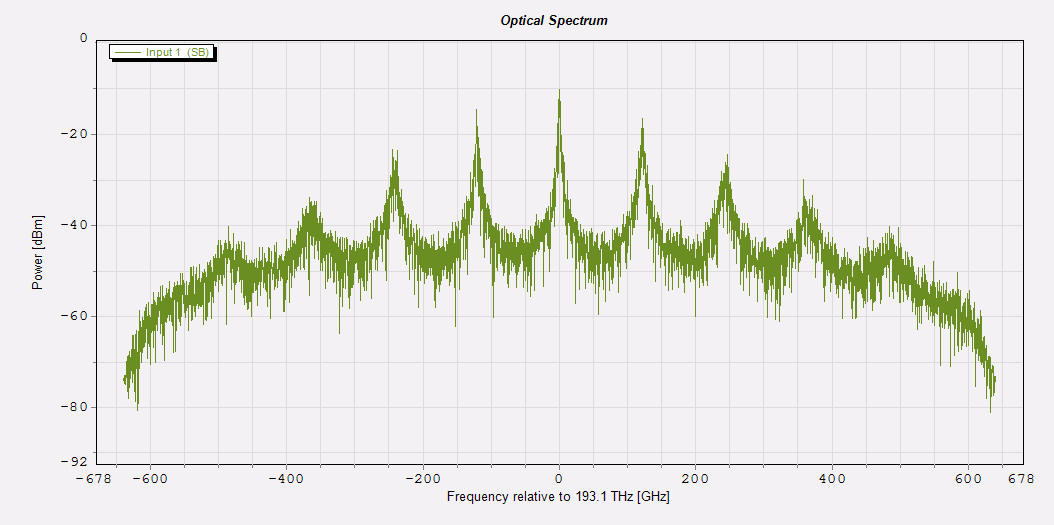
\includegraphics[width=12cm]{Tx1_11.png}\\
  \caption{Laser output spectrum.}
  \label{Tx1_11}
\end{figure}

\begin{figure}[!ht]
  \centering
  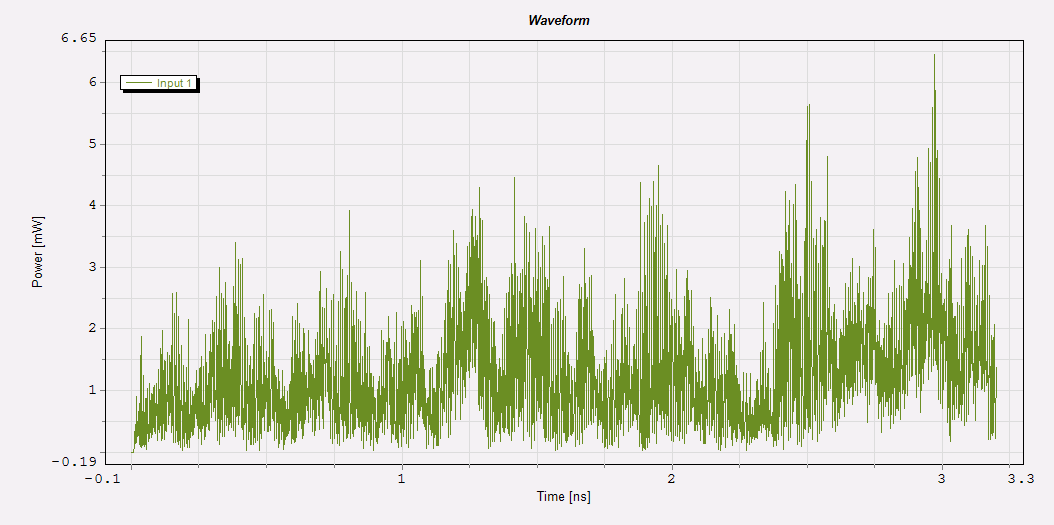
\includegraphics[width=12cm]{Tx1_12.png}\\
  \caption{Laser output waveform.}
  \label{Tx1_12}
\end{figure}

By observing the spectrum we can notice that there are cavity modes: as the gain is not constant over all the bandwidth we have a dominant mode
in correspondence of the central frequency.


We now reduce the gain of the optical amplifier (we set it at 2 dB) and we run the simulation again.
In Figure \ref{Tx1_13} and \ref{Tx1_14} are shown the results.

\begin{figure}[!ht]
  \centering
  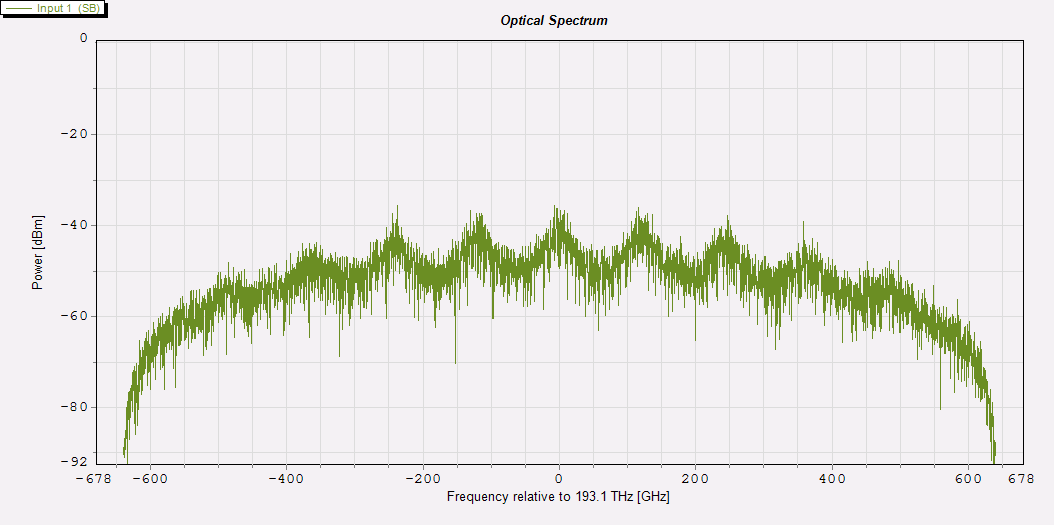
\includegraphics[width=12cm]{Tx1_13.png}\\
  \caption{Laser output spectrum (reduced gain).}
  \label{Tx1_13}
\end{figure}

\begin{figure}[!ht]
  \centering
  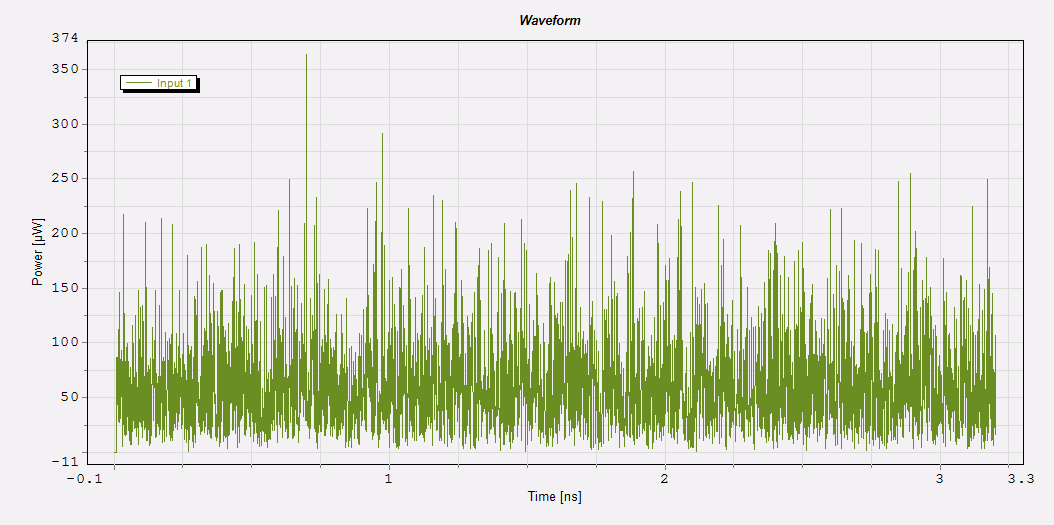
\includegraphics[width=12cm]{Tx1_14.png}\\
  \caption{Laser output waveform (reduced gain).}
  \label{Tx1_14}
\end{figure}

The peaks of the optical spectrum are attenuated and the waveform looks like a noise signal.
This is due to the fact that, decreasing the gain of the
optical amplifier, the losses in the cavity and the ones due to the reflectors are significant respect to the power of the laser itself.
To have lasing, in fact, we have to satisfy two conditions: one regards phase, and the other is about gain. The last one has a limit value known as
threshold gain. Reducing the gain we obtain a behaviour that is closer to spontaneous emission rather than stimulated emission.


\subsection*{Question 1.2}
Now we increase the gain of the optical amplifier (we set it at 6 dB) and we run the simulation again.
In Figure \ref{Tx1_15} and \ref{Tx1_16} are shown the spectrum and the temporal waveform of the laser output.

\begin{figure}[!ht]
  \centering
  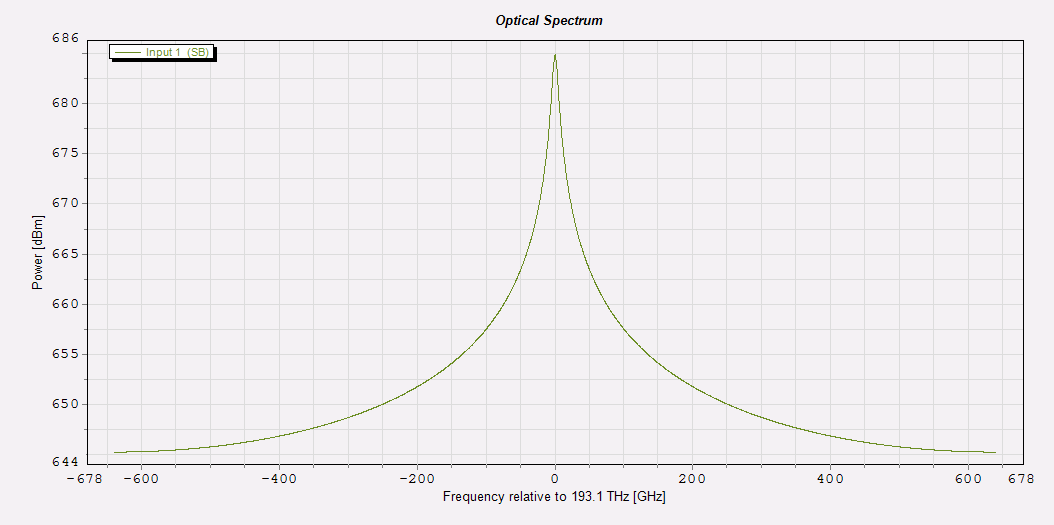
\includegraphics[width=12cm]{Tx1_151.png}\\
  \caption{Laser output spectrum (augmented gain).}
  \label{Tx1_15}
\end{figure}

\begin{figure}[!ht]
  \centering
  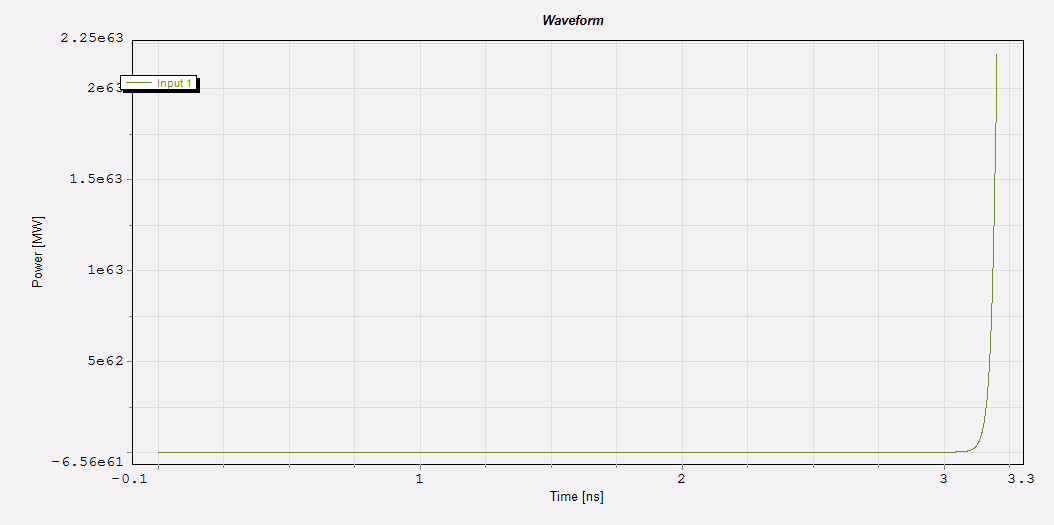
\includegraphics[width=12cm]{Tx1_16.png}\\
  \caption{Laser output waveform (augmented gain).}
  \label{Tx1_16}
\end{figure}

Now the output spectrum presents a very big peak, the waveform is zero until the time 3.15 ns and then jumps to an huge value.
This phenomenon doesn't occur in semiconductor lasers because at laser threshold there is only one laser mode and above threshold
the gain remains constant (it saturates).

\newpage
\section*{Exercise 2: Fabry-Perot Laser}
Now we study the characteristics of continuous wavelength (CW) FP lasers. We use a Bulk FP laser driven by a DC current source and a facet reflectivity
equal to 0.32. We analyse the optical spectrum by using an optical spectrum analyser (OSA).

\subsection*{Question 2.1}
In Figure \ref{Tx1_21} is shown the optical spectrum of the FP laser output.

\begin{figure}[!ht]
  \centering
  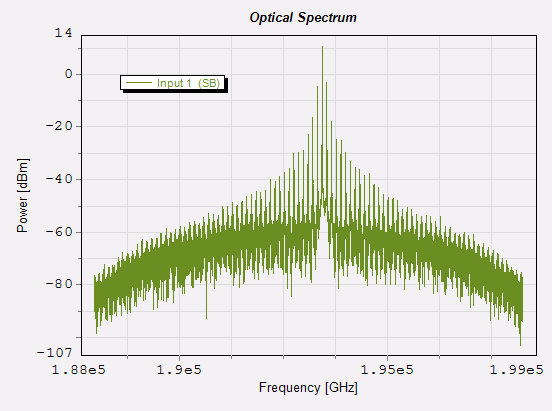
\includegraphics[width=12cm]{Tx1_21.png}\\
  \caption{Laser output spectrum.}
  \label{Tx1_21}
\end{figure}

The spectrum presents equally spaced peaks, that are the cavity modes. These are attenuated according to the curve gain.
To compute the bandwidth of the laser modes we have to use the envelope of the spectrum.
To obtain an approximate envelope we measure some peaks values and then we linearly interpolate them.
The measured values are reported in Table \ref{tab}.

\begin{table}[ht!]
  \begin{center}
    \begin{tabular}{|c|c|}
      \specialrule{.1em}{.05em}{.05em}
	 Frequency [GHz] & Power [dBm]\\
	 \hline
	193202.5 & -16.34\\
	\hline
	193315.3125 & -4.84\\
	\hline
	193428.125 & 10.26\\
	\hline
	193540.9375 & -3.40\\
	\hline
	193653.75 & -18.79\\
      \specialrule{.1em}{.05em}{.05em}
    \end{tabular}
  \end{center}
\caption{Peak powers.}
\label{tab}
\end{table}

In Figure \ref{Tx1_22} is shown the interpolation result.
The bandwidth of the laser modes, computed at -10 dB respect to the peak value, is nearly 100 GHz.
The bandwidth value is quite large: this is a limiting factor in dispersive media.
In fact dispersion is wavelength dependent and limits the maximum bit-rate and the transmission length.


\begin{figure}[!ht]
  \centering
  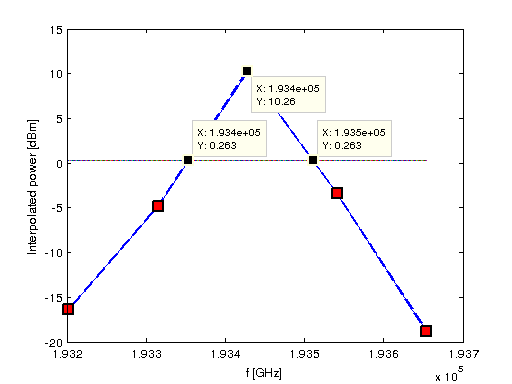
\includegraphics[width=12cm]{Tx1_22.png}\\
  \caption{Laser output spectrum (interpolation).}
  \label{Tx1_22}
\end{figure}


\newpage
\subsection*{Question 2.2}
The aim is to calculate the laser cavity length and check if the result is the same as the simulation parameter, that is $3.5 \cdot 10^{-4} \ m$.
The refractive index of the laser material is $n=3.7$.
The longitudinal mode separation $\Delta \nu$ is the frequential interval between two consecutive frequencies that correspond to a peak value.
These frequencies are reported in Table \ref{tab} and so we find: $\Delta \nu = 112.8125$ GHz.
The laser cavity length is obtained using the following equation:
$$ l = \frac{c}{2 n \Delta \nu}$$
by substituting the values we find $l = 3.5936 \cdot 10^{-4} \ m$, that is very close to the simulation parameter.



\section*{Exercise 3: L-I Curve of Laser Output}
Now we look at the relationship between optical output power and Fabry Perot laser diode drive current.

\subsection*{Question 3.1}
We sweep the laser drive current from 0 to 60 mA, with steps of 5 mA, and we measure the optical output power.
The interface reflection coefficient is set to 0.32.
In Figure \ref{Tx1_31} is shown the simulation result.

The curve looks like the one of a diode characteristic.
At low diode currents (less 20 mA) it is possible to notice that the output power is nearly zero.
In fact the laser is working in the spontaneous emission region.
To obtain the lasing threshold we have to find the line passing by the points of the stimulated emission region curve,
and take the value that correspond to a zero power.
In Figure \ref{Tx1_32} is shown the result: the value of the threshold is nearly 18 mA.

\begin{figure}[!ht]
  \centering
  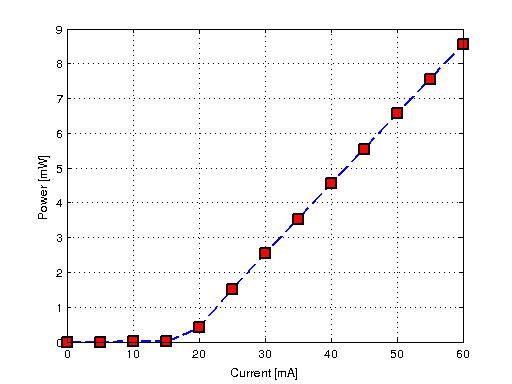
\includegraphics[width=12cm]{Tx1_31.png}\\
  \caption{L-I curve.}
  \label{Tx1_31}
\end{figure}

\begin{figure}[!ht]
  \centering
  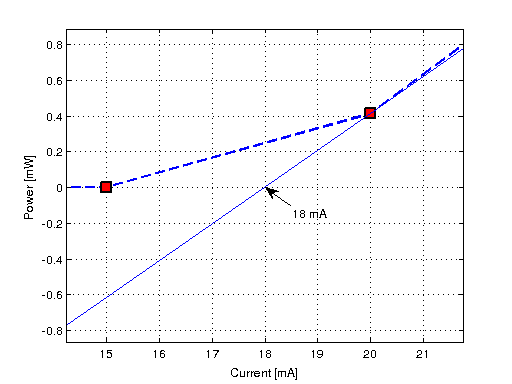
\includegraphics[width=12cm]{Tx1_32.png}\\
  \caption{L-I threshold.}
  \label{Tx1_32}
\end{figure}


\subsection*{Question 3.2}
Now we change the parameter ``interface reflection coefficient'' of the laser and we plot the simulation result.
In Figure \ref{Tx1_33} is shown the graph obtained using the values 0.2 and 0.5: we can notice that the new thresholds are respectively 20 and 15 mA.
We can deduce that, increasing the facet reflectivity, the threshold current decreases.

\begin{figure}[!ht]
  \centering
  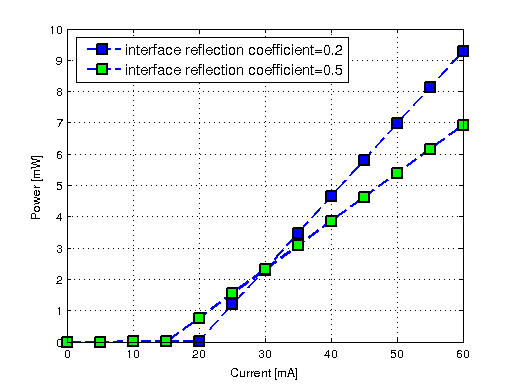
\includegraphics[width=12cm]{Tx1_33.png}\\
  \caption{L-I curves.}
  \label{Tx1_33}
\end{figure}


The external differential quantum efficiency ``h'' is defined as the number of photons emitted per radiative electron-hole pair recombination above
threshold. It is proportional to dP/dI, that is the slope of the L-I curve.
The average values of dP/dI are the following:   0.1138, 0.1118 and  0.0950 (respectively for 0.2, 0.32 and 0.5 interface reflection coefficient).
The efficiency decreases when the reflection coefficient increases.
In the Table \ref{tab2} are summarized the results.

\begin{table}[ht!]
  \begin{center}
    \begin{tabular}{|c|c|c|}
      \specialrule{.1em}{.05em}{.05em}
	 Reflection coefficient & $I_{th}$ & dP/dI\\
	 \hline
	0.2 & 20 &   0.1138\\
	0.32 & 18 & 0.1118\\
	0.5 & 15 &  0.0950\\
      \specialrule{.1em}{.05em}{.05em}
    \end{tabular}
  \end{center}
\caption{Results.}
\label{tab2}
\end{table}



\newpage
\section*{Exercise 4: Temporal Dynamics of FP Laser}
We simulate the dynamics of FP lasers.

\subsection*{Question 4.1}
We plot the carrier density and waveform of the laser output over a observation time of 800 ps.
We divide the observation time in four intervals, separated by the points in time when the carrier density has either a local minimum or maximum.
In Figure \ref{4_1} is shown the first time interval: it goes from 0 to 581 ps. During this time the carrier density increases until it reaches
a maximum. The output power increases as well.
\newpage

\begin{figure}[!ht]
  \centering
  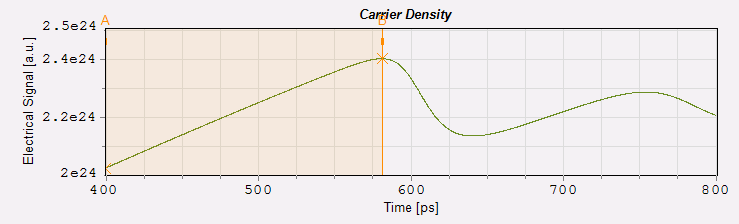
\includegraphics[width=12cm]{4_1cd.png}\\
  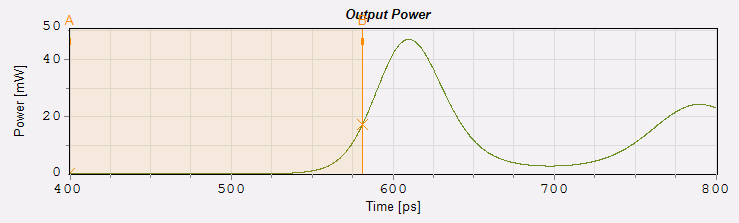
\includegraphics[width=12cm]{4_1pw.png}\\
  \caption{Carrier density and output power, first interval.}
  \label{4_1}
\end{figure}

In Figure \ref{4_2} is shown the second time interval: it goes from 581 to 640 ps.
The carrier density decreases until it reaches a minimum, the output power increases until it reaches a maximum and then decreases.
\begin{figure}[!ht]
  \centering
  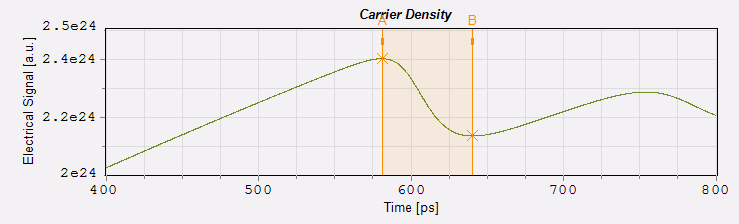
\includegraphics[width=12cm]{4_2cd.png}\\
  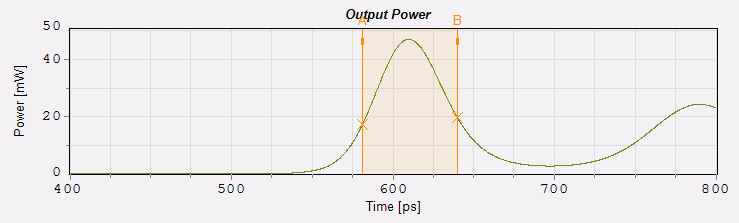
\includegraphics[width=12cm]{4_2pw.png}\\
  \caption{Carrier density and output power, second interval.}
  \label{4_2}
\end{figure}

In Figure \ref{4_3} is shown the third time interval: it goes from 640 to 753 ps.
The carrier density increases until it reaches a maximum and the output power first decreases and then increases as well.
\begin{figure}[!ht]
  \centering
  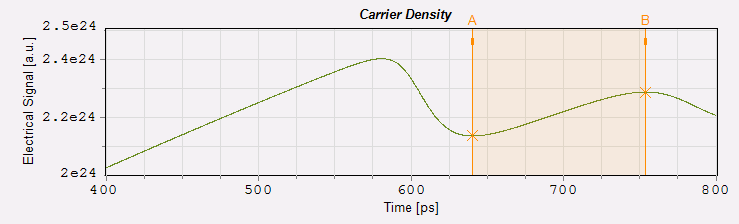
\includegraphics[width=12cm]{4_3cd.png}\\
  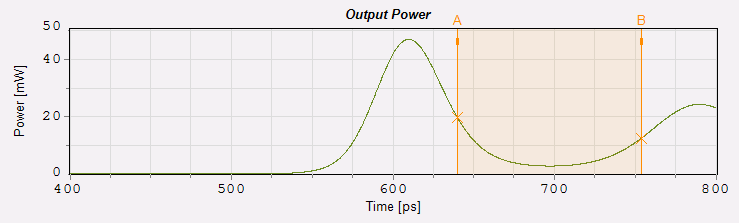
\includegraphics[width=12cm]{4_3pw.png}\\
  \caption{Carrier density and output power, third interval.}
  \label{4_3}
\end{figure}

In Figure \ref{4_4} is shown the fourth time interval: it goes from 753 to 800 ps.
The carrier density decreases while the output power first increases and then decreases.
\begin{figure}[!ht]
  \centering
  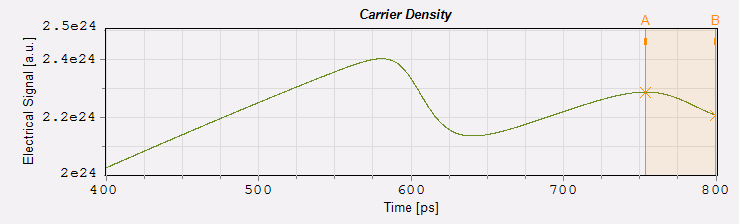
\includegraphics[width=12cm]{4_4cd.png}\\
  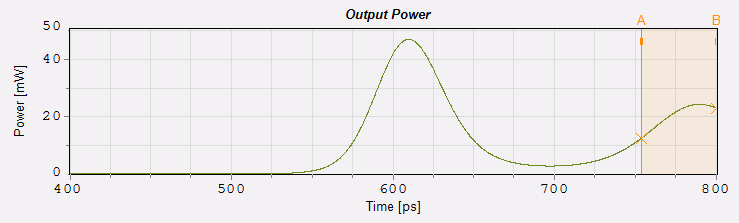
\includegraphics[width=12cm]{4_4pw.png}\\
  \caption{Carrier density and output power, fourth interval.}
  \label{4_4}
\end{figure}

When the carrier density increases or decreases the output power increases or decreases as well, but with a delay.
This is due to the fact that the laser presents a turn-on delay between the injection of the current and the generation of the light.
In fact, to have stimulated emission, the population of excited and ground state must be inverted (by electrical pumping) and this
requires a certain amount of time.


\newpage
\section*{Exercise 5: Resonant Frequency and Drive Current}
We investigate the relationship between the resonant frequency and the drive current of the laser.

\subsection*{Question 5.1}
We sweep the drive current between 0 A and 0.06 A.
In Figure \ref{5_curve} is shown the L-I curve of the laser output. From Figure \ref{5_1} to \ref{5_6} are shown the laser output waveforms
for current values from 0 up to 0.06 A.

\begin{figure}[!ht]
  \centering
  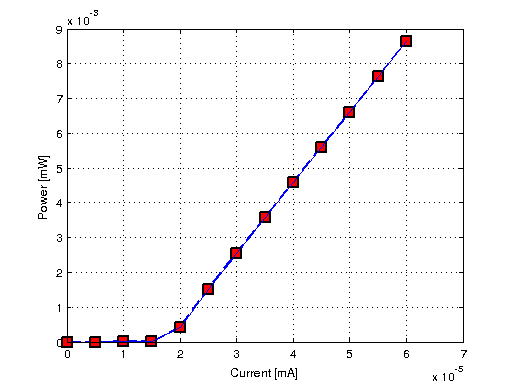
\includegraphics[width=12cm]{5_curve.png}\\
  \caption{L-I curve.}
  \label{5_curve}
\end{figure}

\begin{figure}[!ht]
  \centering
  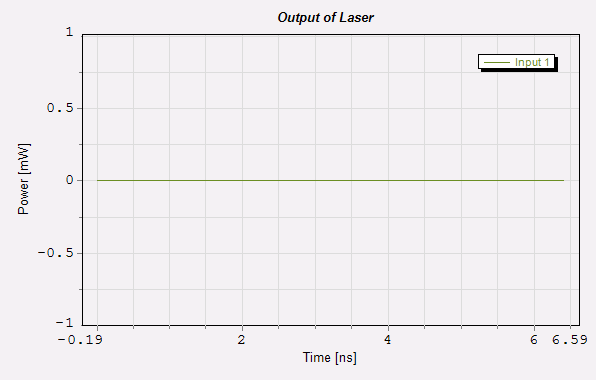
\includegraphics[width=12cm]{5_2.png}\\
  \caption{Laser output waveform, I=0 A.}
  \label{5_1}
\end{figure}

\begin{figure}[!ht]
  \centering
  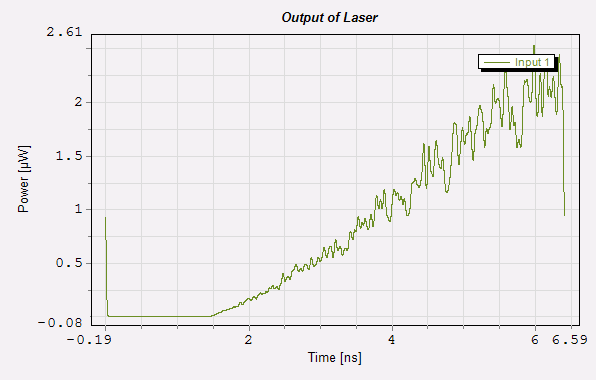
\includegraphics[width=12cm]{5_4.png}\\
  \caption{Laser output waveform, I=0.01 A.}
  \label{5_2}
\end{figure}

\begin{figure}[!ht]
  \centering
  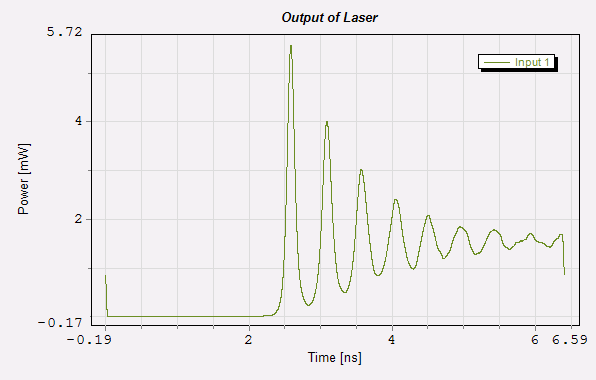
\includegraphics[width=12cm]{5_6.png}\\
  \caption{Laser output waveform, I=0.02 A.}
  \label{5_3}
\end{figure}

\begin{figure}[!ht]
  \centering
  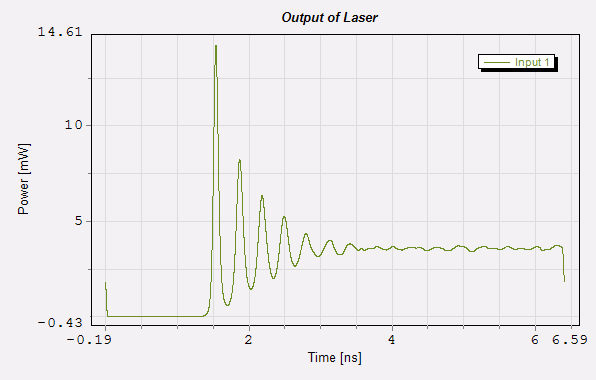
\includegraphics[width=12cm]{5_8.png}\\
  \caption{Laser output waveform, I=0.03 A.}
  \label{5_4}
\end{figure}

\begin{figure}[!ht]
  \centering
  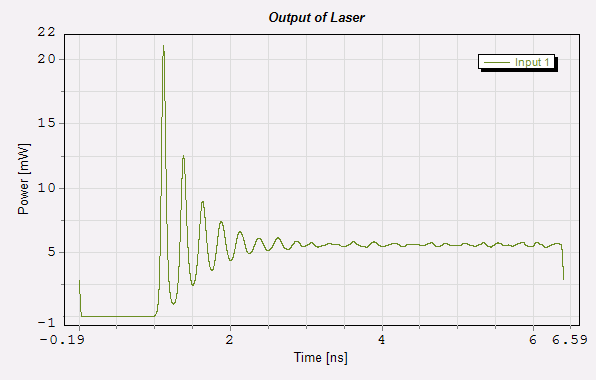
\includegraphics[width=12cm]{5_10.png}\\
  \caption{Laser output waveform, I=0.04 A.}
  \label{5_5}
\end{figure}

\begin{figure}[!ht]
  \centering
  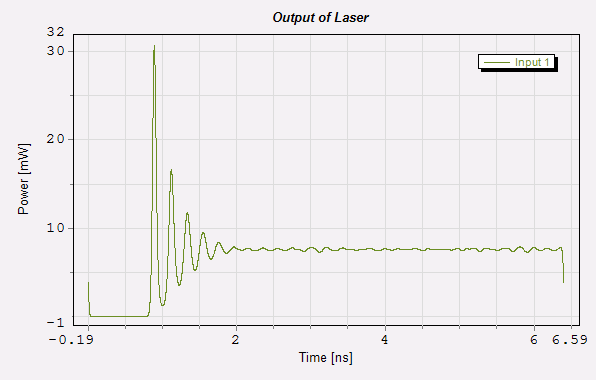
\includegraphics[width=12cm]{5_12.png}\\
  \caption{Laser output waveform, I=0.06 A.}
  \label{5_6}
\end{figure}

The resonant frequency is defined as $f_r=1/\Delta t$, where $\Delta t$ is the period of the first oscillation of the laser output waveform.
In Table \ref{tab3} are reported the measured resonant frequencies, for different values of drive current I.

\begin{table}[ht!]
  \begin{center}
    \begin{tabular}{|c|c|}
      \specialrule{.1em}{.05em}{.05em}
	 I [A] & $f_r$ [GHz]\\
	 \hline
	0.02 & 1.2355\\
	0.03 & 2.5937\\
	0.04 & 3.3818\\
	0.05 & 4.0635\\
	0.06 & 4.6715\\
      \specialrule{.1em}{.05em}{.05em}
    \end{tabular}
  \end{center}
\caption{Resonant frequencies.}
\label{tab3}
\end{table}

In Figure \ref{5_fr2} is shown the plot of ${f_r}^2$ versus $I/(I_{th}-1)$, the value $I_{th}$ is measured from Figure \ref{5_curve}
and it is nearly 18 mA.

\begin{figure}[!ht]
  \centering
  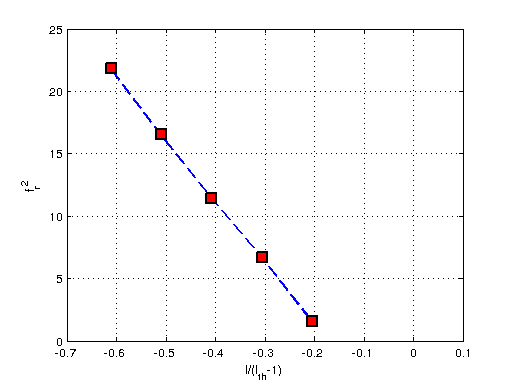
\includegraphics[width=12cm]{5_fr2.png}\\
  \caption{${f_r}^2$ versus $I/(I_{th}-1)$.}
  \label{5_fr2}
\end{figure}


\newpage
\section*{Exercise 6: DFB Laser}
We study distributed feedback (DFB) lasers. These lasers use a grating in the laser cavity to generate one single mode.

\subsection*{Question 6.1}
We use a DFB laser with quarter-wave-shifted grating. The grating model is set to ``grating'', the interface reflection coefficient is
set to $10^{-12}$ and the grating phase shift is equal to 90.
In Figure \ref{6_1} is shown the spectrum of the laser output. There is one cavity mode, the signal mode bandwidth measured at -10 dB from the
maximum is nearly 240 MHz. In the Fabry Perot laser the bandwidth was nearly 100 GHz, that is three orders of magnitude higher.
DFB lasers are suited for WDM systems because of their narrow occupied bandwidth. In this way it is possible to exploit better the fiber capacity,
by sending more channels (spaced in frequency) at the same time.

\begin{figure}[!ht]
  \centering
  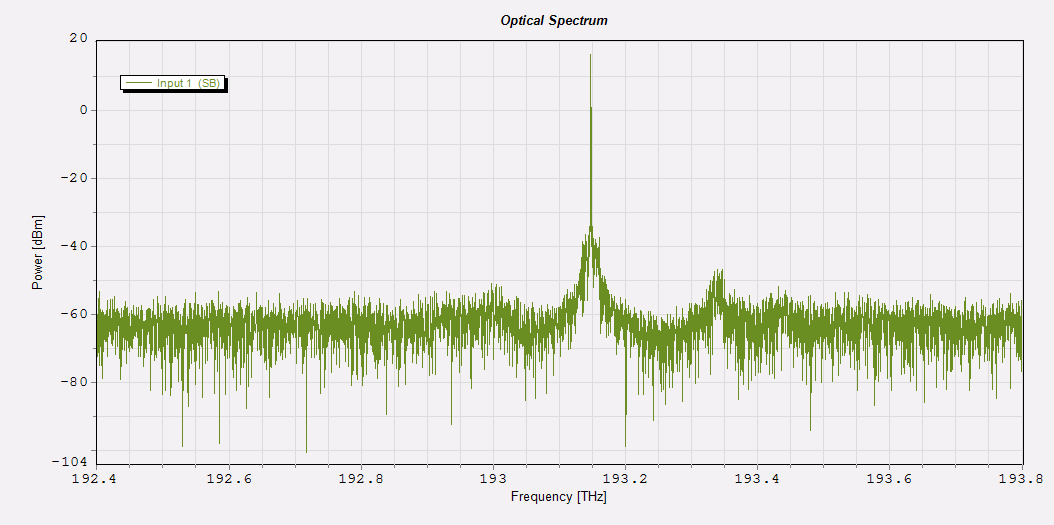
\includegraphics[width=12cm]{6_1.png}\\
  \caption{DFB laser, power spectrum.}
  \label{6_1}
\end{figure}

In Figure \ref{6_2} and \ref{6_3} are shown the spectra obtained with a grating phase shift of $0^\circ$ and $180^\circ$ respectively.
In both cases appear two peaks around 193.1 and 193.3 THz, the spectra are similar (it changes the attenuation).

\begin{figure}[!ht]
  \centering
  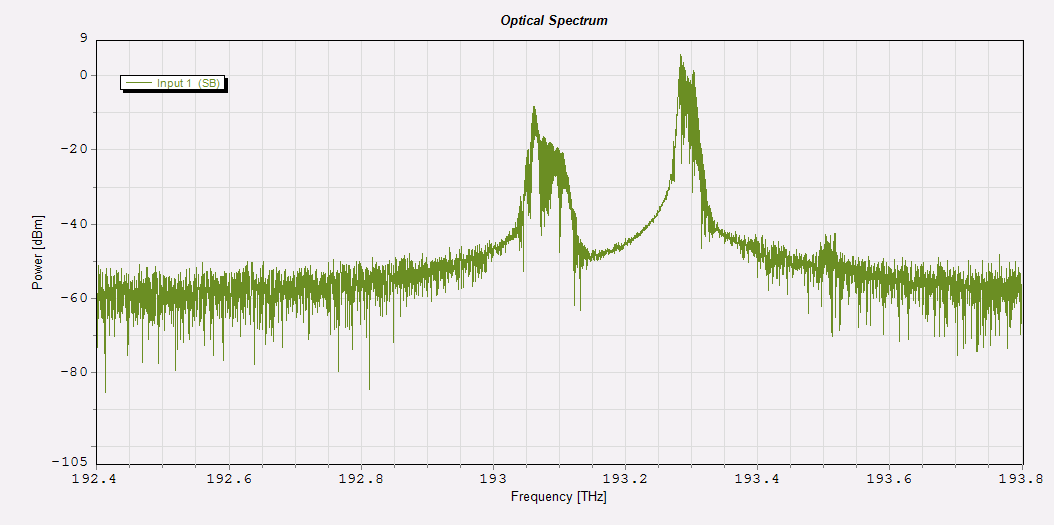
\includegraphics[width=12cm]{6_2.png}\\
  \caption{DFB laser, power spectrum, zero grating phase shift.}
  \label{6_2}
\end{figure}

\begin{figure}[!ht]
  \centering
  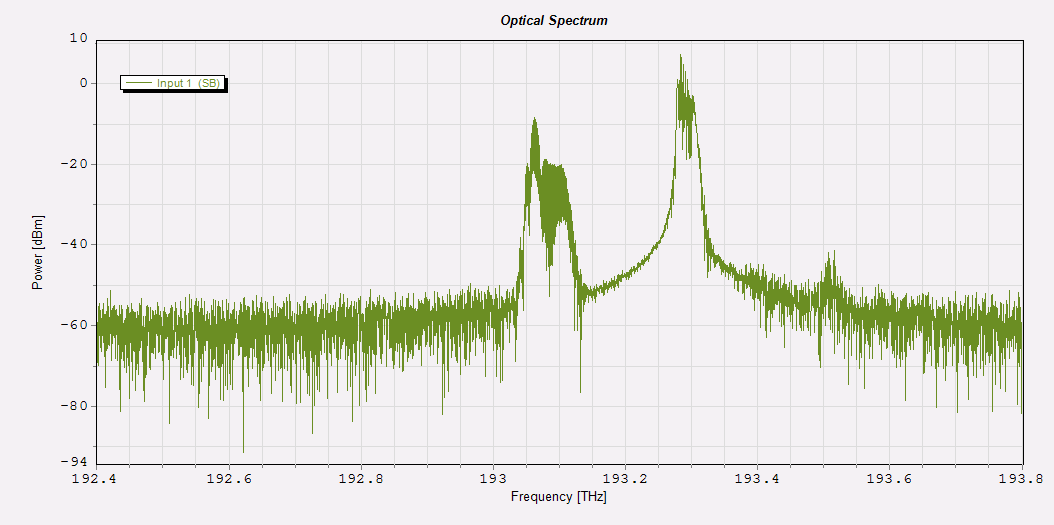
\includegraphics[width=12cm]{6_3.png}\\
  \caption{DFB laser, power spectrum, $180^\circ$ grating phase shift.}
  \label{6_3}
\end{figure}

\subsection*{Question 6.2}
To better understand why the mode of the DFB laser has a very small width, we plot the laser output and frequency for the same values of
grating phase shift as before.
In Figure \ref{6_4}, \ref{6_5} and \ref{6_6} are shown the simulation results.
When the phase shift is $90^\circ$, the power and the chirp in time domain look like a quasi constant value. This translates into a peak
in frequency domain (as we can see in Figure \ref{6_1}).
When the phase shift is zero or $180^\circ$ the power and the chirp in time domain have a periodic behaviour, and this translates into a
broadening of the spectrum (as we can see in Figure \ref{6_2} and \ref{6_3}).

\begin{figure}[!ht]
  \centering
  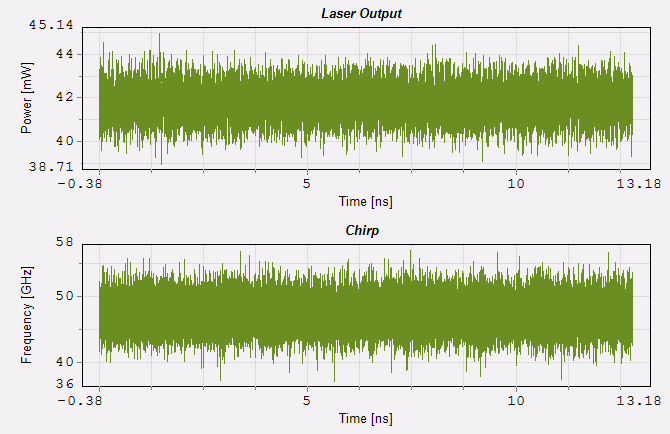
\includegraphics[width=12cm]{6_4.png}\\
  \caption{DFB laser, power spectrum, $90^\circ$ grating phase shift.}
  \label{6_4}
\end{figure}

\begin{figure}[!ht]
  \centering
  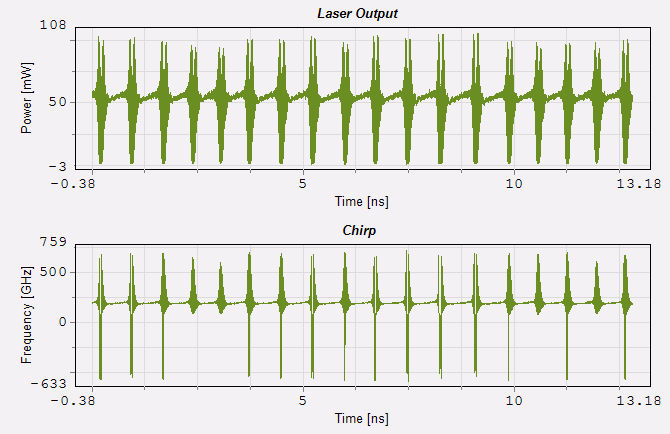
\includegraphics[width=12cm]{6_5.png}\\
  \caption{DFB laser, power spectrum, $0^\circ$ grating phase shift.}
  \label{6_5}
\end{figure}

\begin{figure}[!ht]
  \centering
  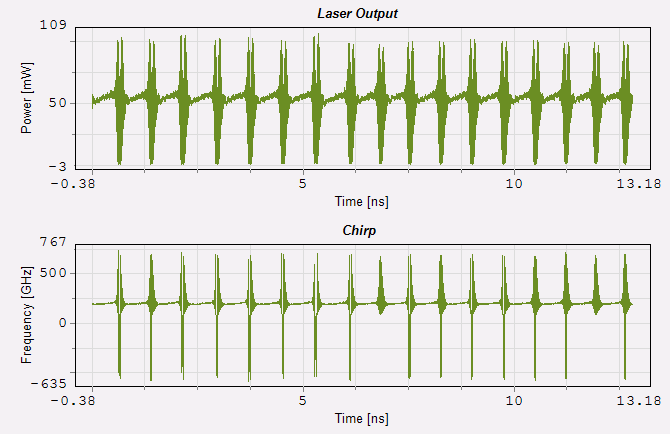
\includegraphics[width=12cm]{6_6.png}\\
  \caption{DFB laser, power spectrum, $180^\circ$ grating phase shift.}
  \label{6_6}
\end{figure}




\newpage
\section*{Exercise 7: Directly Modulated DFB Laser}
We perform a direct modulation to a DFB laser.

\subsection*{Question 7.1}
We set the NRS signal to ``ONE'' and we run the simulation. In Figure \ref{7_1one} is shown the optical spectrum.

\begin{figure}[!ht]
  \centering
  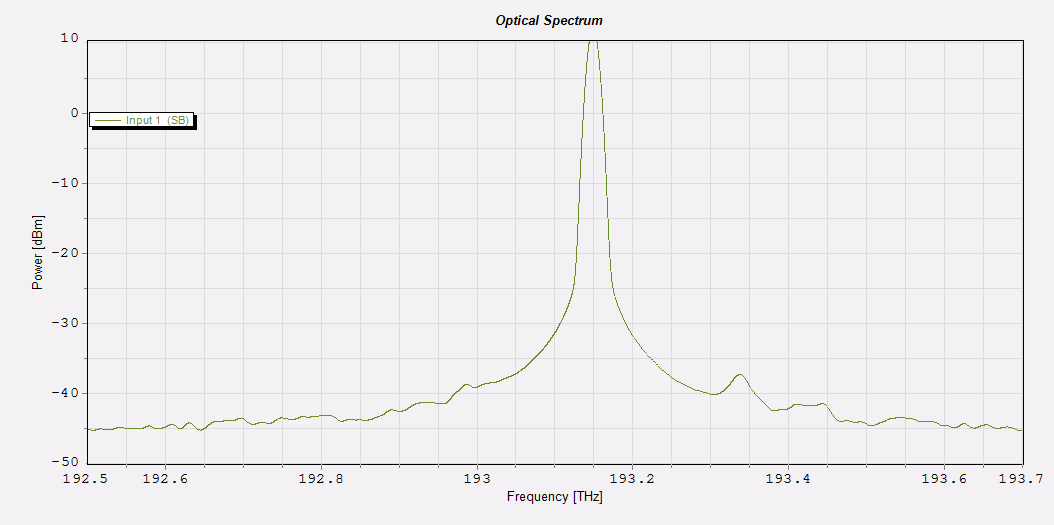
\includegraphics[width=12cm]{7_1one.png}\\
  \caption{Optical spectrum, ONE.}
  \label{7_1one}
\end{figure}

In Figure \ref{7_1} is shown the optical spectrum obtained by setting the NRS signal to ``PRBS''.

\begin{figure}[!ht]
  \centering
  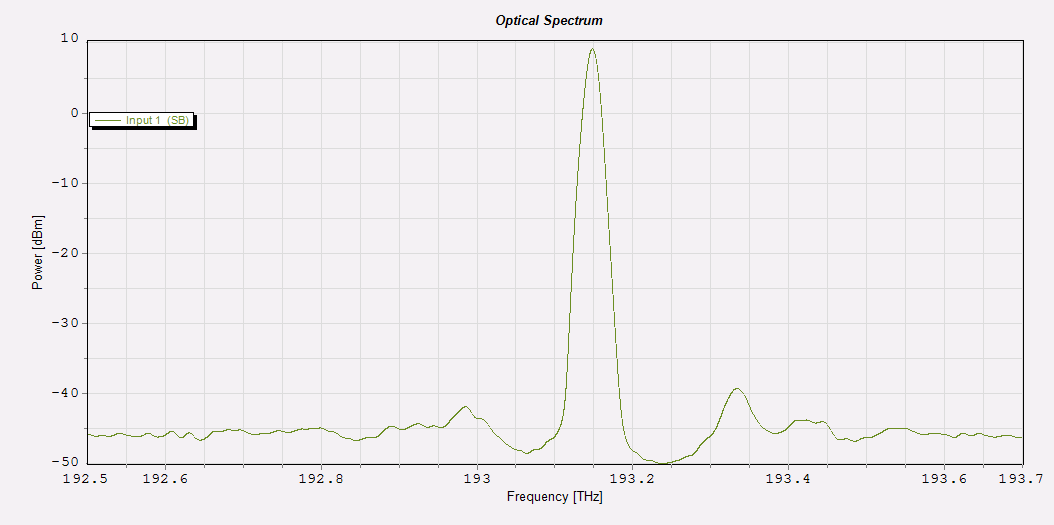
\includegraphics[width=12cm]{7_1.png}\\
  \caption{Optical spectrum, PRBS.}
  \label{7_1}
\end{figure}

In the case of modulation equal to ``ONE'' the laser transmits a sequence made of all ``1'' pulses. The coding is a NRZ (non return to zero), so the
output power in time domain is a constant. In frequency this translates into a delta centred at the modulation frequency.

When the modulation is ``PRBS'' (pseudo-random binary sequence) the laser transmits a random sequence of ``1'' and ``0''. The NRZ coding, every time
that encounters a transition ``01'' or ``10'' modulates the light according to the transition. This causes the spectrum to have a wider lobe and
two zeros at the side of the lobe itself.

\subsection*{Question 7.2}
In Figure \ref{7_2} are shown the power waveform and the chirp for the PRBS NRZ modulation.
When we have a transition from ``0'' to ``1'', at the leading edge of the pulses we have an overshoot. This is due to the direct modulation of the laser
with the sequence of zeros and ones. The phenomenon is the one studied in Exercise 5: when the laser is turned on (it is fed with a drive current),
before reaching the regime value, it has an oscillating behaviour (relaxation oscillations). Also when we have a transition from ``1'' to ``0'' we have an analog phenomenon:
the output oscillates, before reaching a stable value.

\begin{figure}[!ht]
  \centering
  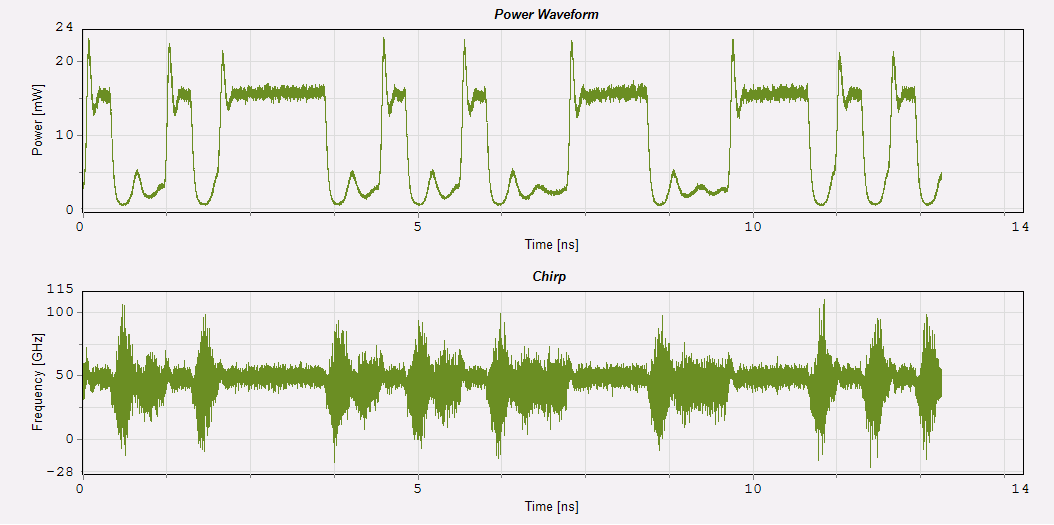
\includegraphics[width=12cm]{7_2.png}\\
  \caption{Power waveform and chirp, PRBS.}
  \label{7_2}
\end{figure}

In Figure \ref{7_punto2} is shown the graph constructed by measuring the laser output peak power P and the value of the chirp $\Delta C$, by varying
the drive current from 0 to 90 mA (in intervals of 20 mA).
The value of $\Delta C$ is obtained by roughly measuring the maximum and minimum values of the chirp function, and subtracting them.
If the power increases (that is 1/P decreases), the values of the chirp increases as well.

\begin{figure}[!ht]
  \centering
  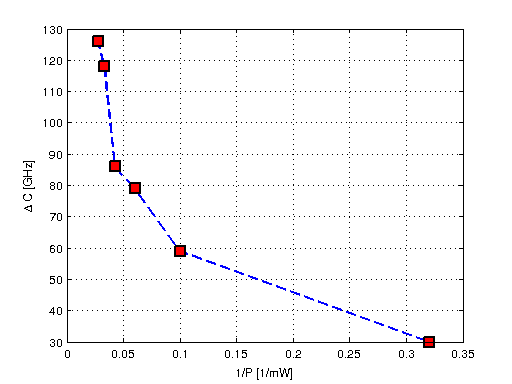
\includegraphics[width=12cm]{7_punto2.png}\\
  \caption{$\Delta C$ versus 1/P.}
  \label{7_punto2}
\end{figure}


\subsection*{Question 7.3}
We set the driver current to 60 mA and we plot the evolution of the carrier density in the DFB laser. In Figure \ref{7_punto32} is shown the
simulation result. We can observe that the evolution of the carrier density follows somehow the one of the power waveform.

\begin{figure}[!ht]
  \centering
  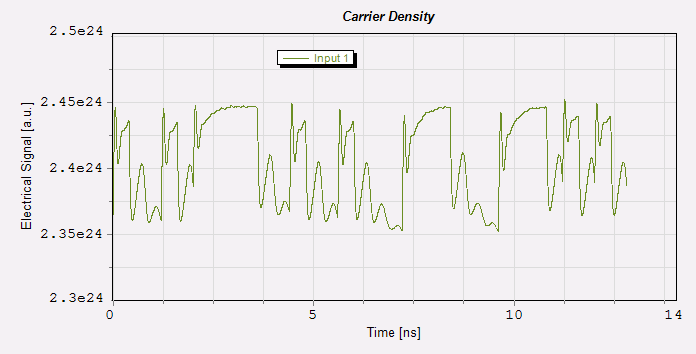
\includegraphics[width=12cm]{7_punto32.png}\\
  \caption{Carrier density evolution.}
  \label{7_punto32}
\end{figure}


\newpage
\section*{Exercise 8: External Modulation and Direct Modulation}
Now we compare the optical signal after external modulation and direct modulation. To externally modulate the laser output, an electro-absorption
(EA) modulator is used.

\subsection*{Question 8.1}
In Figure \ref{8_1} are shown the power spectrum and the chirp of the directly modulated DFB laser.
It is possible to notice that there are oscillations on the transitions from ``0'' to ``1'' state, and also peaks after the laser is turned off.

\begin{figure}[!ht]
  \centering
  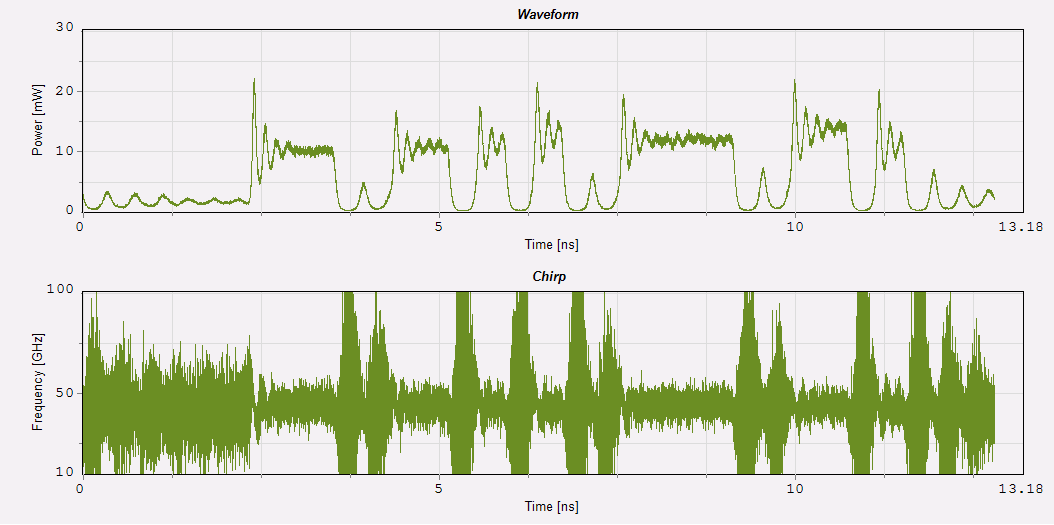
\includegraphics[width=12cm]{8_1.png}\\
  \caption{Power waveform and chirp, direct modulation.}
  \label{8_1}
\end{figure}

\subsection*{Question 8.2}
In Figure \ref{8_2} are shown the power spectrum and the chirp of the externally modulated DFB laser.
We can observe that there are no oscillations nor at the leading edges nor at the trailing edges of the pulses.
This is due to the fact that the laser is always turned on, and the light is modulated at its output.
The chirp has the same behaviour for all the simulation time, while with the direct modulation, the chirp waveform varied more.

\begin{figure}[!ht]
  \centering
  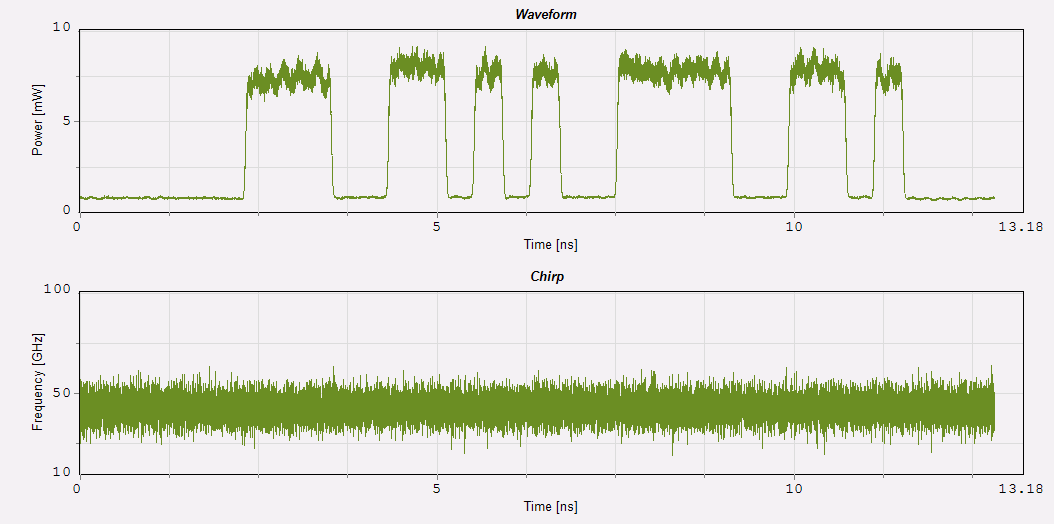
\includegraphics[width=12cm]{8_2.png}\\
  \caption{Power waveform and chirp, external modulation.}
  \label{8_2}
\end{figure}





\newpage
\section*{Exercise 9: Responsivity of PIN and APD}
We show the relationship between the photocurrent generated from PIN or APD photodiodes and input optical power.
The optical input light for both lasers is generated by a continuous wave (CW) laser, the photocurrent generated is first averaged and then visualized.

\subsection*{Question 9.1}
We sweep the input optical power of the photodetector by controlling the attenuator value (we decrease the attenuation from 20 to 0 dB, with steps of 2 dB).
In Figure \ref{9_pin} and \ref{9_apd} are shown the plots of the averaged photocurrent, generated from both PIN and APD photodiode respectively,
versus input optical power.

\begin{figure}[!ht]
  \centering
  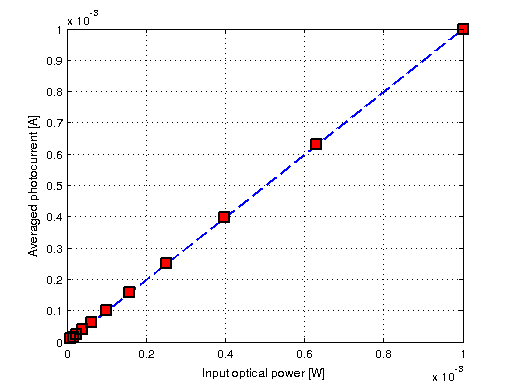
\includegraphics[width=12cm]{9_pin.png}\\
  \caption{Averaged photocurrent versus input optical power, PIN photodiode.}
  \label{9_pin}
\end{figure}

\begin{figure}[!ht]
  \centering
  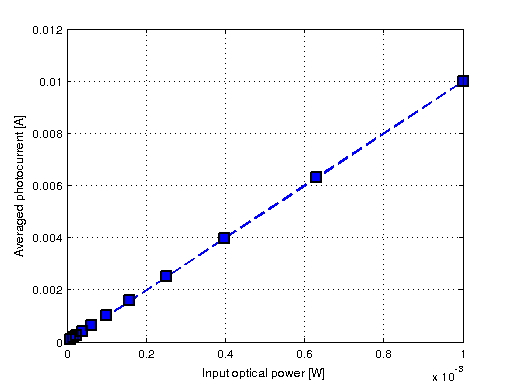
\includegraphics[width=12cm]{9_apd.png}\\
  \caption{Averaged photocurrent versus input optical power, APD photodiode.}
  \label{9_apd}
\end{figure}

The relationship obtained is linear.
The responsivity of the photodiodes can be estimated by using the following equation $$R=\frac{I}{P}$$
where I is the generated photocurrent and P is the received power. By substituting the values obtained in the simulation (and reported on the graphs),
we find:
\begin{itemize}
  \item $R_{PIN}=0.9998 \ [A/W]$
  \item $R_{APD}=10.0049 \ [A/W]$
\end{itemize}

In the simulation, the responsivity was set to 1 for both the photodiodes and the avalanche multiplication factor was set to 10.
The $R_{PIN}$ value is very similar to the simulation one, but the $R_{APD}$ one is nearly 10 times bigger.
This is due to the fact that APD photodetectors are characterized by the avalanche multiplication factor that causes them
to have a higher responsivity respect to PIN photodetectors.


\end{document}